% !TEX root = ../Thesis.tex
\chapter{Top quark physics}\label{ch:TopQuark}

The third generation of quarks was first proposed by Kobayashi and Maskawa in a paper published in 1973~\cite{Theory:CKMKobayashiMaskawa} as a way to explain the $CP$ violation observed in kaon decays~\cite{Evidence}. The existence of the third generation in the quark sector was confirmed when the lighter of the two constituents, the $b$-quark, was discovered in 1977~\cite{Top:bQuarkDiscovered}. 

Due to its large mass, direct production of the top quark required the construction of very powerful accelerators. However, its mass was constrained in precision electroweak measurements at LEP in 1995 to be~\cite{Top:TopMassLEP}:
%
\begin{equation}
  m_{\textrm{top}}=\num{174}\;^{+\;21.5}_{-\;25.5}\;\si{GeV}
\end{equation}

The top quark was then discovered by the CDF and D0 experiments at Fermilab in 1995~\cite{Top:ObservationCDF,Top:ObservationD0} and then observed at CERN again in 2010~\cite{TopQuark:FirstTopAtATLAS,TopQuark:FirstTopAtCMS}.

The large mass of the top quark makes it a very interesting object of study. The current world average for the mass of the top quark, based on results from Tevatron and the LHC~\cite{Theory:PDGBooklet}, is
%
\begin{equation*}
  m_{t}=173.07\pm0.52\stat\pm0.72\syst\si{\GeV}
\end{equation*}

Due to its mass the top quark has an extremely short lifetime $\tau\approx\SI{0.5e-24}{\second}$, too short to interact via the strong force and hadronize into a bound state~\cite{Theory:TopQuarkDecayTooQuickly}. Instead the top quark decays weakly producing a $W$ boson and a $b$-quark almost exclusively. This allows experimentalists to directly study the properties of a bare quark. An impossibility with the other quarks which bind with other quarks to form hadrons. Measurement of top quark properties (mass, charge, forward-backward asymmetry, couplings, etc\ldots) forms a large part of high energy physics research. Measurement of these properties provide rigorous tests of the SM, and could point towards the existence of new physics or exclude some BSM theories.

From an experimental perspective, top quark decays produce a very interesting signature with leptons, jets and missing energy due to the escaping neutrino\footnote{Neutrinos do not interact with the detector material and thus escape without being detected, missing energy is described in more detail in Chapter~\ref{ch:Detector}}. Therefore, the study of top quark decays relies on all parts of a general purpose detector such as ATLAS or CMS\@. Finally, \ttbar\ pair production also is a major background for many other SM and BSM searches, so understanding this process well is fundamental to almost all areas of HEP research.

\section{Top quark production}\label{sec:top_quark_production}

Top quarks can be produced in two ways: single top production and \ttbar\ pair production. In the SM the dominant top quark pair production mechanism proceeds via the strong force. The production cross section of $pp\rightarrow\ttbar$ depends on the mass of the top $m_{t}$, the centre of mass energy $\sqrt{s}=2E_{\textrm{beam}}$ and the fraction of the momentum taken by the partons\footnote{The constituents of hadrons: quarks and gluons} of the colliding protons.

In order to produce a \ttbar\ pair the total energy carried by the interacting partons must be larger than twice the mass of the top. Let us define the effective centre of mass energy $\hat{s}$ which reflects the true amount of energy available for interaction. Given two colliding partons, denoted $i$ and $j$ carrying $x_i$ and $x_j$ fractions of the centre of mass energy $\cme$, then
%
\begin{equation}
  \hat{s} = x_{i}\cme x_{j}\cme = x_{i}x_{j}s
\end{equation}
%
assuming that both partons carry the same fraction of the total energy, i.e. $x_i\approx x_j$ then the minimum value of $x$ required for \ttbar\ production is
%
\begin{equation}
  x\approx\frac{2m_t}{\sqrt{s}}  
\end{equation}

At the LHC the minimum threshold at $\cme=\SI{7}{\TeV}(\SI{14}{\TeV})$ is approximately 0.05(0.025). At such low values of $x$ the fraction of proton momentum carried by the gluons is large~\cite{TopQuark:HATHORCrossSection} and thus gluon fusion interactions dominate as can be seen in Figure~\ref{fig:TopMSTWNLOPDFs}.

\begin{figure}[htbp]
  \centering
    \includegraphics[width=0.75\textwidth]{PartTopQuark/Plots/mstw2008nlo68cl_allpdfs.eps}
    \caption{MSTW 2008 NLO parton distribution functions.}\label{fig:TopMSTWNLOPDFs}
\end{figure}

Gluon fusion processes represent $\num{80}(\num{90})\si{\percent}$ of the total cross section, with the remainder contribution coming from quark pair annihilation. The Feynman diagrams for these interactions are shown in Figure~\ref{fig:TopQuarkProduction}. The theoretical inclusive \ttbar\ production cross section at the LHC has been calculated at NNLO level to be $\sigma_{t\bar{t}}=158\;^{-\;12.2}_{+\;13.5}\;\si{\pico\barn}$~\cite{TopPair} at \cmsS, and $\sigma_{t\bar{t}}=252.9\;^{+\;6.4}_{-\;8.6}\pm11.7\;\si{\pico\barn}$~\cite{TopQuark:CrossSection8TeV} for \cmsE.
%
\begin{figure}[htbp]
  \centering
  \begin{minipage}[][][t]{.47\textwidth}
    \centering
    % !TEX root = ../../Thesis.tex
\begin{fmffile}{TopProdStraightgg2tt}
\fmfframe(5,17)(20,17) {
\begin{fmfgraph*}(150,70)
\fmfleft{gluon1,gluon2}
\fmfright{tbar,top}
\fmf{gluon}{gluon1,v1}
\fmf{gluon}{gluon2,v2}
\fmf{fermion}{tbar,v1}
\fmf{fermion,tension=0}{v1,v2}
\fmf{fermion}{v2,top}
\fmflabel{$g$}{gluon1} \fmflabel{$t$}{top}
\fmflabel{$g$}{gluon2} \fmflabel{$\overline{t}$}{tbar}
\end{fmfgraph*}
}
\end{fmffile}
    \subcaption{Gluon fusion (t-channel)}
  \end{minipage}
  \,
  \begin{minipage}[][][t]{.47\textwidth}
    \centering
    % !TEX root = ../../Thesis.tex
\begin{fmffile}{TopProdCrossGG2ttbar}
\fmfframe(5,17)(20,17) {
\begin{fmfgraph*}(150,70)
\fmfleft{i1,i2}
\fmfright{o1,o2}
\fmf{gluon}{v1,i1}
\fmf{phantom}{v1,o1} % Invisible rubber band
\fmf{gluon}{v2,i2}
\fmf{phantom}{v2,o2} % also invisible rubber band
\fmf{fermion,tension=0}{v1,v2}
% These are visible, but have no tension.
\fmf{fermion,tension=0}{o2,v1}
\fmf{fermion,tension=0}{v2,o1}
\fmflabel{$g$}{i1}
\fmflabel{$g$}{i2}
\fmflabel{$t$}{o1}
\fmflabel{$\overline{t}$}{o2}
\end{fmfgraph*}
}
\end{fmffile}
    \subcaption{Gluon fusion (u-channel)}
  \end{minipage}
  
  \begin{minipage}[][][t]{.47\textwidth}
    \centering
    % !TEX root = ../../Thesis.tex
\begin{fmffile}{TopProdgg2g2ttbar}
\fmfframe(5,17)(5,17) {
\begin{fmfgraph*}(150,70)
\fmfleft{gluon1,gluon2}
\fmfright{top1,top2}
\fmf{gluon}{v1,gluon1}
\fmf{gluon}{v1,gluon2}
\fmf{gluon,label=$g$,l.d=10}{v2,v1}
\fmf{fermion}{top1,v2,top2}
\fmflabel{$g$}{gluon1} \fmflabel{$t$}{top2}
\fmflabel{$g$}{gluon2} \fmflabel{$\bar{t}$}{top1}
\end{fmfgraph*}
}
\end{fmffile}
    \subcaption{Gluon fusion (s-channel)}
  \end{minipage}
  \,
  \begin{minipage}[][][t]{.47\textwidth}
    \centering
    % !TEX root = ../../Thesis.tex
\begin{fmffile}{TopProdqq2ttbar}
\fmfframe(5,17)(5,17) {
\begin{fmfgraph*}(150,70)
\fmfleft{q,qbar}
\fmfright{tbar,top}
\fmf{fermion}{qbar,v1,q}
\fmf{gluon,label=$g$,l.d=10}{v2,v1}
\fmf{fermion}{tbar,v2,top}
\fmflabel{$q$}{q} \fmflabel{$t$}{top}
\fmflabel{$\bar{q}$}{qbar} \fmflabel{$\bar{t}$}{tbar}
\end{fmfgraph*}
}
\end{fmffile}
    \subcaption{Quark pair annihilation}
  \end{minipage}
  \,
  \caption{The leading order Feynman diagrams for \ttbar\ production.}\label{fig:TopQuarkProduction}
\end{figure}

Single top production occurs via the weak force almost exclusively through the $Wtb$ vertex since $|V_{tb}|\gg|V_{ts}|,|V_{td}|$. At LO there are several production mechanisms for single-top events:

\begin{itemize}
  \item Weak quark-antiquark annihilation forming a \W\ which subsequently decays into a $t\bar{b}$ (Figure~\ref{fig:TopSingleSChannel}).
  \item The so-called $tW$ production, where a $b$-quark absorbs a gluon and decays to a top quark and $W$ boson (Figure~\ref{fig:TopSingletWChannel}).
  \item $b$-quark scattering off a $W$ boson, where the $b$ comes from gluon splitting (Figure~\ref{fig:TopSingleqtbChannel}) or from the proton (Figure~\ref{fig:TopSingleqtChannel}).
\end{itemize}

As top quark pair production can proceed via the strong force it occurs overwhelmingly more often than single top production. The inclusive cross sections for $pp\rightarrow t+X$ at the LHC have been estimated at NLO, and are summarized in Table~\ref{tab:TopQuarkPredictionCrossSection}. The production cross section of \ttbar\ is approximately two times larger than the single-top cross section.

\begin{table}[htbp]
  \centering
  \begin{tabular}{@{}lcc@{}}
  \toprule
  Process & \multicolumn{2}{c}{cross section at [\si{\pico\barn}]} \\
  \cmidrule{2-3}
  & $\sqrt{s}=\SI{7}{\TeV}$ & $\sqrt{s}=\SI{8}{\TeV}$ \\
  \midrule
  Single top $\sigma$ (t-chan)  & $66\pm2$         & $87\pm3$     \\
  Single top $\sigma$ (Wt)      & $15.6\pm1.2$     & $22.2\pm1.5$ \\
  \bottomrule
  \end{tabular}
  \caption[Summary of the predicted SM single top production and top pair production cross sections at the LHC for \cmsS\ and \cmsE.]{Summary of the predicted SM single top production~\cite{Kidonakis:2012rm} and top pair production~\cite{Czakon:2013goa} cross sections at the LHC for \cmsS\ and \cmsE.}\label{tab:TopQuarkPredictionCrossSection}
\end{table}
~%
\begin{figure}[htpb]
  \centering
  \begin{minipage}[][][t]{.47\textwidth}
    \centering
    % !TEX root = ../../Thesis.tex
\begin{fmffile}{TopSingleTopSChannel}
\fmfframe(5,17)(20,17) {
\begin{fmfgraph*}(150,70)
\fmfleft{quark,antiquark}
\fmfright{top,bbar}
\fmf{fermion}{quark,v1,antiquark}
\fmf{boson,label=$W$}{v1,v2}
\fmf{fermion}{bbar,v2,top}
\fmflabel{$q$}{quark} \fmflabel{$t$}{top}
\fmflabel{$\overline{q'}$}{antiquark} \fmflabel{$\overline{b}$}{bbar}
\fmfdot{v1,v2}
\end{fmfgraph*}
}
\end{fmffile}
    \subcaption{s-channel}\label{fig:TopSingleSChannel}
  \end{minipage}
  \,
  \begin{minipage}[][][t]{.47\textwidth}
    \centering
    % !TEX root = ../../Thesis.tex
\begin{fmffile}{TopSingleTWChannel}
\fmfframe(5,17)(20,17) {
\begin{fmfgraph*}(150,70)
\fmfleft{gluon,b}
\fmfright{top,W}
\fmf{gluon}{gluon,v1}
\fmf{fermion}{b,v1}
\fmf{fermion,label=$b$}{v1,v2}
\fmf{fermion}{v2,top}
\fmf{boson}{v2,W}
\fmflabel{$g$}{gluon} \fmflabel{$t$}{top}
\fmflabel{$b$}{b} \fmflabel{$W$}{W}
\end{fmfgraph*}
}
\end{fmffile}
    \subcaption{$tW$-channel}\label{fig:TopSingletWChannel}
  \end{minipage}

  \begin{minipage}[][][t]{.47\textwidth}
    \centering
    % !TEX root = ../../Thesis.tex
\begin{fmffile}{TopSingleQtb}
\fmfframe(5,17)(18,17) {
\begin{fmfgraph*}(150,70)
\fmfleft{glu1,quark}
\fmfright{bbar,top,qprime}
\fmf{fermion}{quark,v1,qprime}
\fmf{gluon}{v3,glu1}
\fmf{fermion}{bbar,v3}
\fmffreeze
\fmf{phantom}{v1,v3}
\fmf{boson,label=$W$}{v1,v2}
\fmf{fermion,label=$b$}{v3,v2}
\fmffreeze
\fmf{fermion}{v2,top}
\fmflabel{$g$}{glu1} \fmflabel{$t$}{top}
\fmflabel{$q$}{quark} \fmflabel{$q'$}{qprime} \fmflabel{$\bar{b}$}{bbar}
\end{fmfgraph*}
}
\end{fmffile}
    \subcaption{Associated with a $q$ and $\bar{b}$}\label{fig:TopSingleqtbChannel}
  \end{minipage}
  \,
  \begin{minipage}[][][t]{.47\textwidth}
    \centering
    % !TEX root = ../../Thesis.tex
\begin{fmffile}{TopSingleqb2qt}
\fmfframe(5,17)(5,17) {
\begin{fmfgraph*}(150,70)
\fmfleft{ib,iq}
\fmfright{ot,oq}
\fmf{fermion}{iq,v1,oq}
\fmf{fermion}{ib,v2,ot}
\fmffreeze
\fmf{boson,label=$W$}{v1,v2}
\fmflabel{$b$}{ib} \fmflabel{$t$}{ot}
\fmflabel{$q$}{iq} \fmflabel{$q'$}{oq}
\end{fmfgraph*}
}
\end{fmffile}
    \subcaption{Associated with a $q$}\label{fig:TopSingleqtChannel}
  \end{minipage}
  \caption{Example Feynman diagrams for single top quark at leading order.}\label{fig:TopSingleProduction}
\end{figure}

\section{Top quark decay modes}\label{sec:top_quark_decay_modes}

The top quark decays almost exclusively into a $W$ boson and a $b$-quark. The world average measured ratio of branching ratios $\Gamma(t\rightarrow Wb)/\Gamma(t\rightarrow Wq(q=b,s,d))$ is \num{0.91(4)}~\cite{Theory:PDGBooklet}. Note that there is some tension between this measured result and the naive expectation from the CKM matrix. The measured value is $2\sigma$ away from the expected CKM result, meaning there is perhaps some room for additional quark generations not accounted for by the CKM matrix.

As the LHC collides proton-proton beams, the overwhelming majority of events produced will feature multiple hadronic \textit{jets}, a stream of particles resulting from the hadronization of quarks in the detector, most of which will originate from ``light'' quarks\footnote{The term light quarks usually refers to quarks in the first two generations. Light jets are those originating from those quarks}. Unlike light hadrons, $B$-hadrons have a sufficiently large lifetime that they travel a certain distance before decaying. Additional features such as the semileptonic decay of $b$-quarks can be exploited to determine the presence of such a quark in the detector. Collectively analysis techniques that permit the detection of $b$-jets are known as \textit{b-tagging}. Top quark pairs will produce two $b$-quarks, making $b$-tagging techniques a central part of any \ttbar\ analysis. More information on $b$-tagging techniques, including the Soft Muon Tagger, is provided in Chapter~\ref{ch:Detector}.

The other part of the top decay, the $W$ boson, is used to classify \ttbar\ events. The $W$ boson can decay leptonically ($W\rightarrow\ell\nu_{\ell}$) or hadronically ($W\rightarrow q\bar{q}'$) driven by the CKM vertex element. The branching ratios of $W$ boson decays are presented in Table~\ref{tab:TopQuakWDecayBranchingRatios}.

\begin{table}[htbp]
  \centering
  \begin{tabular}{@{}cS[table-format=2.2(2)]@{}}
    \toprule
    $W$ decay to & {Branching ratio [\si{\percent}]} \\
    \midrule
    $e+\nu$      & 10.75(13) \\
    $\mu+\nu$    & 10.57(15) \\
    $\tau+\nu$   & 11.25(20) \\
    Hadrons      & 67.60(27) \\
    \bottomrule
  \end{tabular}
  \caption[Branching ratios of $W$ boson decay.]{Branching ratios of $W$ boson decay. \textbf{Hadrons} refers to all possible combinations of $q\bar{q}'$ where $\bar{q}'$ denotes the antiquark of a flavour different to that of the first quark~\cite{Theory:PDGBooklet}.}\label{tab:TopQuakWDecayBranchingRatios}
\end{table}

Top quark pair events are labelled as ``dilepton'', ``all-hadronic'' or ``lepton plus jets'' depending on the combination of $W$ boson decays present. The probability for a \ttbar\ event to be of a given type is dependent on the branching ratios of $W$ boson decays shown previously. As can be seen from Figure~\ref{fig:TopQuarkDecayModes} the all-hadronic events dominate, followed by the lepton plus jets and dilepton. Each event type requires a different analysis approach due to their distinct backgrounds, branching ratio, detector signature and reconstruction requirements. Note that some lepton plus jets analyses do not explicitly treat taus directly. Nevertheless tau decays enter into these analysis via its decay to an electron or muon. Thus the true branching ratio is marginally smaller than that shown in the Figure~\ref{fig:TopQuarkDecayModes}.

\begin{figure}[tbhp]
  \centering
  \includegraphics[width=0.75\textwidth]{PartTopQuark/Diagrams/TopQuarkDecayPie.pdf}
  \caption[Branching ratios of all possible \ttbar\ decays.]{Branching ratios of all possible \ttbar\ decays. These probabilities are based on the branching ratios of $W$ boson decay shown in Table~\ref{tab:TopQuakWDecayBranchingRatios}. Note that the lepton plus jets branching ratio here includes all three leptons.}\label{fig:TopQuarkDecayModes}
\end{figure}

The all-hadronic final state includes four light quarks which will hadronize to form four light flavour (LF) jets and two $b$-quarks leading to two $b$-jets. Due to the large hadronic activity the all-hadronic channel is very challenging. As mentioned before, hadronic collisions produce events with a large number of jets in the final state. The background to the all-hadronic channel are therefore very high. As shown in Figure~\ref{fig:TopQuarkDecayModes} the all-hadronic channel has the largest branching ratio of the three.

The dilepton final state includes two leptons, large missing energy from two neutrinos which escape the detector and two $b$-jets. In contrast to the all-hadronic channel, dilepton events are very clean due to the presence of leptons and missing energy, however the branching ratio is very small and reconstruction of the top quarks is challenging due to the presence of the two neutrinos. Finally, the lepton plus jets channel has a larger branching ratio than the dilepton while having a distinct signature with a lepton and missing energy as well as LF jets and $b$-jets.

Lepton plus jets analyses do have some acceptance to $\tau$ events, but they are not usually treated as the signal lepton. The $\tau$ lepton is unstable and decays primarily via the weak force producing hadrons in the final state. Events with $\tau$ leptons enter lepton plus jets analyses when the $\tau$ decays leptonically into a muon or electron. The reconstruction of $\tau$ leptons is a complex task and $\tau$ plus jet events are treated separately with dedicated analyses. An example of the full lepton plus jets chain is shown in Figure~\ref{fig:TopQuarkFullLPlusJets}.

\begin{figure}[p]
  \centering
  \includegraphics[height=0.65\textheight]{PartTopQuark/Diagrams/atlas-2010-063-fig_09.png}
  \caption{Example event display of a dilepton \ttbar\ event recorded by ATLAS\@. The electrons are shown as yellow energy depositions in the green EM calorimeter. These are associated with a green and orange upward-pointing tracks in the ID\@. Some hadronic activity is noted in the red hadronic calorimeter on the opposite side.}\label{fig:TopQuarkEventDisplay}
\end{figure}

The lepton plus jets channel has the advantage of a more distinct signature than the all-hadronic event as well as a suffering from less background. The branching ratio of lepton plus jets event is also approximately twice that of the dilepton channel. As a result the lepton plus jets channel has been chosen as the focus of this thesis.

\begin{figure}[htbp]
  \centering
  \begin{minipage}[][][t]{.60\textwidth}
  % !TEX root = ../../Thesis.tex
\begin{fmffile}{TopQuarkLeptonPlusJetsFull}
\fmfframe(5,17)(20,17) {
\begin{fmfgraph*}(200,200)
\fmfstraight
\fmfleft{dummy1,gluon1,gluon2,dummy2}
\fmfright{q,antiq,b,antib,lep,nu}
\fmf{gluon}{v1,gluon1}
\fmf{gluon}{v1,gluon2}
\fmf{gluon,label=$g$,l.d=10}{v2,v1}
\fmf{fermion,label=$t$,l.d=-14,tension=0.5}{top,v2}
\fmf{fermion,label=$\bar{t}$,tension=0.5}{v2,antitop}
\fmf{fermion,tension=0,tension=0}{antib,antitop}
\fmf{boson,label=$W$,tension=0}{antitop,leptonicW}
\fmf{fermion}{nu,leptonicW,lep}
\fmf{fermion,tension=0}{b,top}
\fmf{boson,label=$W$,tension=0}{hadronicW,top}
\fmf{fermion,tension=0}{antiq,hadronicW,q}
\fmflabel{$g$}{gluon1}
\fmflabel{$g$}{gluon2}
\fmflabel{$\bar{b}$}{antib}
\fmflabel{$b$}{b}
\fmflabel{$\bar{q}'$}{q}
\fmflabel{$q$}{antiq}
\fmflabel{$\ell$}{lep}
\fmflabel{$\nu_{\ell}$}{nu}
\end{fmfgraph*}
}
\end{fmffile}
  \end{minipage}
  \caption[Feynman diagram of lepton plus jets channel including \ttbar\ production via gluon fusion and decay with a leptonically decaying $W^{+}$.]{Feynman diagram of lepton plus jets channel including \ttbar\ production via gluon fusion and decay with a leptonically decaying $W^{+}$. All other production mechanisms are also considered and the final state where the $W^{-}$ decays leptonically is also taken into account.}\label{fig:TopQuarkFullLPlusJets}
\end{figure}

\section{Latest developments in top physics}

This section discusses a few of the latest measurements in the area of top quark pair production with a focus on LHC results. Top quark decays provide the only probe to study the properties of a bare quark. Measurements of its properties provide a stringent test of the SM and could show hints of new physics from BSM theories. Moreover, due to its final state signature top quark pair production, particularly in the lepton plus jets channel, form the background to many searches for new physics.  All parts of the detector are utilized in the reconstruction of $\ell$+jets events and so it is possible to use these events to tune or \textit{calibrate} analysis and reconstruction techniques.

\subsubsection{Cross section measurement}

Measurement of the production cross section of the top quark at different centre of mass energies\footnote{The production cross section is dependent on the centre of mass energy of the collision.} is a benchmark test of the SM. Any statistically significant deviation from the predicted value could point to the presence of new physics. Some BSM theories posit the existence of particles which could decay to produce a \ttbar\ pair. If such theory is correct this would be observed in an increase in the cross section measured away from the predicted SM value. Precise knowledge of the cross section is also vital from an experimental perspective, for example when attempting to reduce and estimate the amount of top quark background present in other analyses. Searches for the Higgs boson exploit many different channels such as $t\bar{t}H\rightarrow t\bar{t}b\bar{b}$ which have \ttbar\ events as a background. The type of events predicted by the BSM theory, supersymmetry (SUSY) include a large amount of missing energy, leptons and jets in the final state. Top quark pair events mimic these processes and constitute a large background.

A summary of all \ttbar\ cross section measurements from the LHC at \cmsS\ is shown in Figure~\ref{fig:TopQuarkPairProductionSummaryLHC} and a comparison against the Tevatron measurement at $\sqrt{s}=\SI{1.96}{\TeV}$ is shown in Figure~\ref{fig:TopQuarkPairProductionComparison}. Early results at \cmsE\ are shown in Figure~\ref{fig:TopQuarkPairProduction8TeV}.

\begin{figure}[htbp]
  \centering
  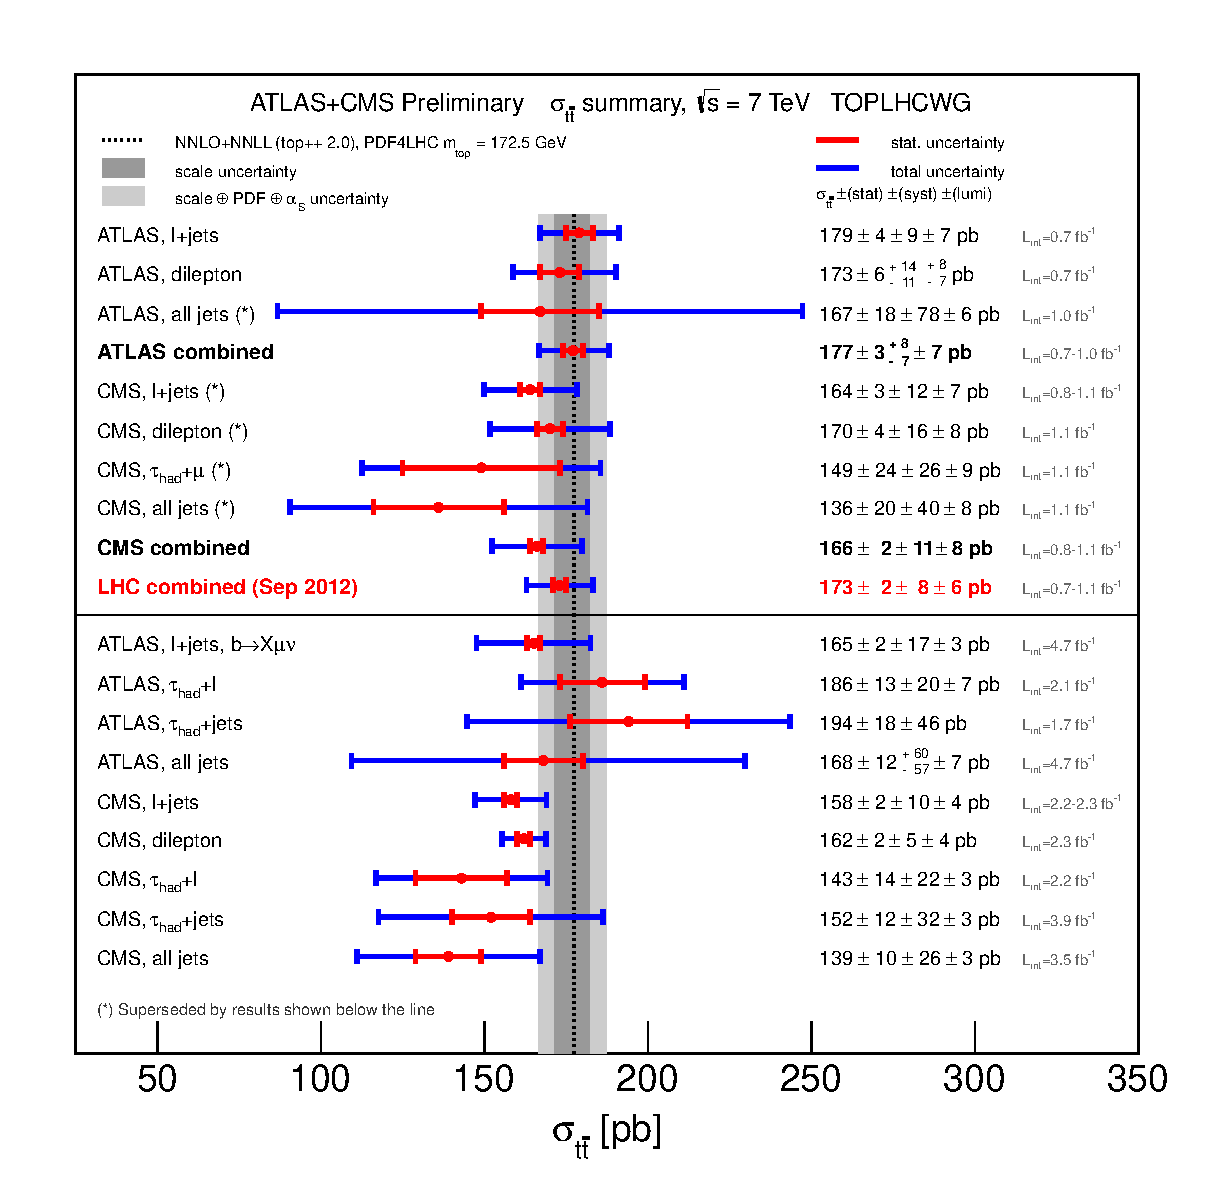
\includegraphics[width=0.75\textwidth]{PartTopQuark/Plots/tt_xsec_7TeV.eps}
  \caption[A summary of all \ttbar\ production cross section measurements performed at the LHC at \cmsS.]{A summary of all \ttbar\ production cross section measurements performed at the LHC at \cmsS~\cite{TopQuark:SummaryPlots}. The theory prediction shown as a dotted black line associated uncertainties as grey bands. The results shown above the black line have been statistically combined, producing the results labelled as \textbf{combined}. Many of these analyses have been superseded and the results are shown below the line. Other analyses performed but not included in the combination are also shown below the line, such as the analysis described in Chapter~\ref{ch:CrossSection}.}\label{fig:TopQuarkPairProductionSummaryLHC}
\end{figure}

\begin{figure}[htbp]
  \centering
  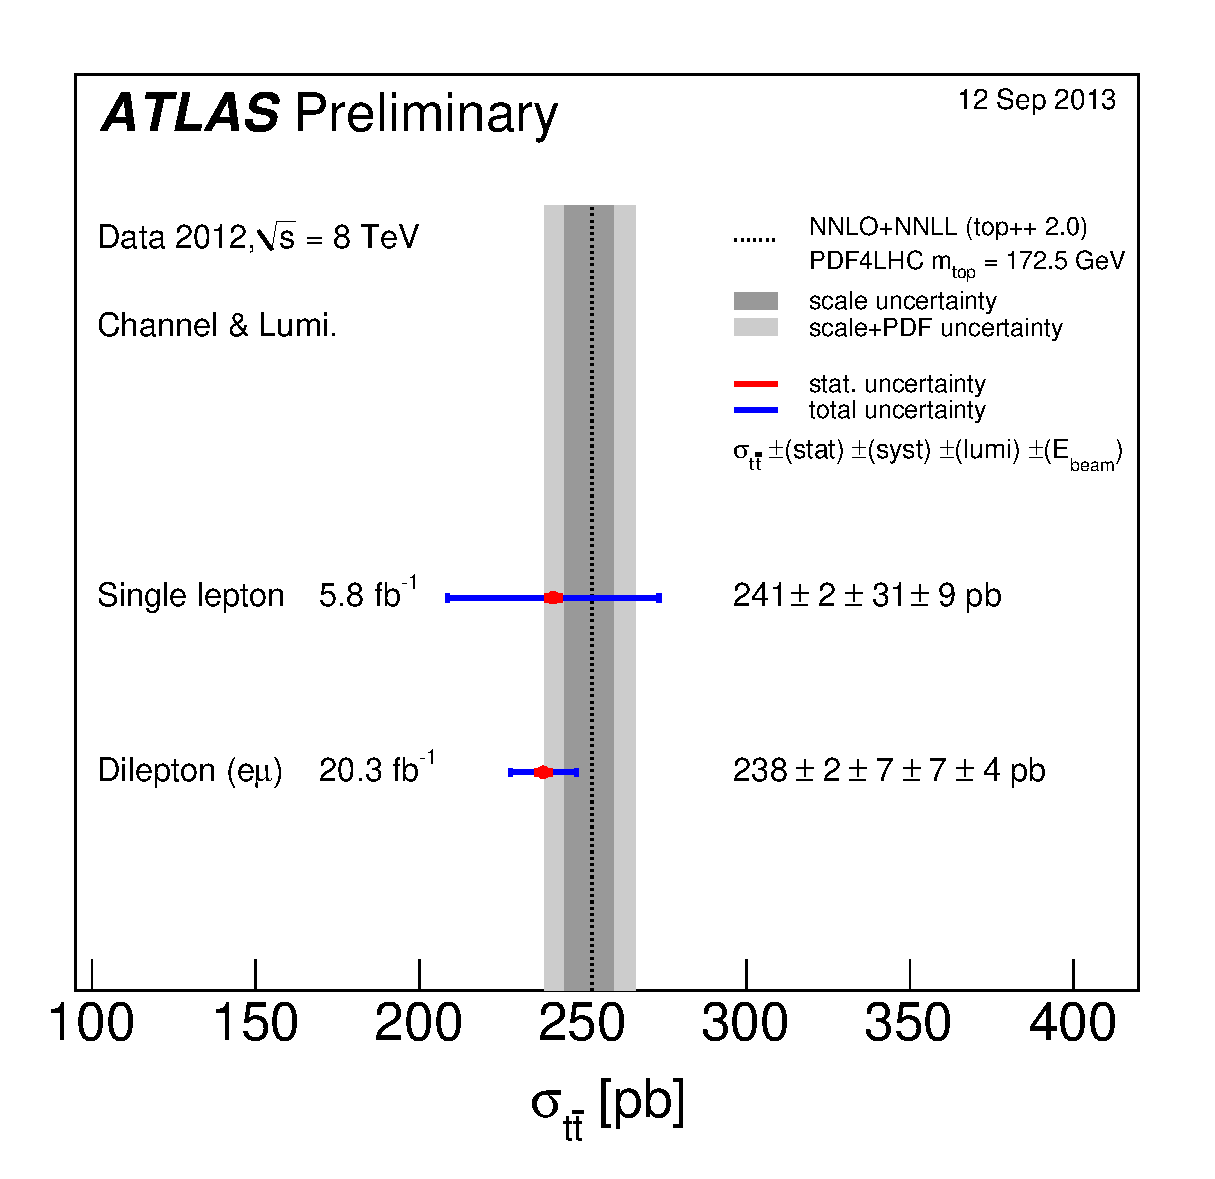
\includegraphics[width=0.75\textwidth]{PartTopQuark/Plots/tt_xsec_8TeV.eps}
  \caption[A summary of all \ttbar\ production cross section measurements performed at the LHC at \cmsE.]{A summary of all \ttbar\ production cross section measurements performed at the LHC at \cmsE~\cite{TopQuark:SummaryPlots}. The theory prediction is shown as a dotted line with associated uncertainties as grey bands.}\label{fig:TopQuarkPairProduction8TeV}
\end{figure}

\begin{figure}[htbp]
  \centering
  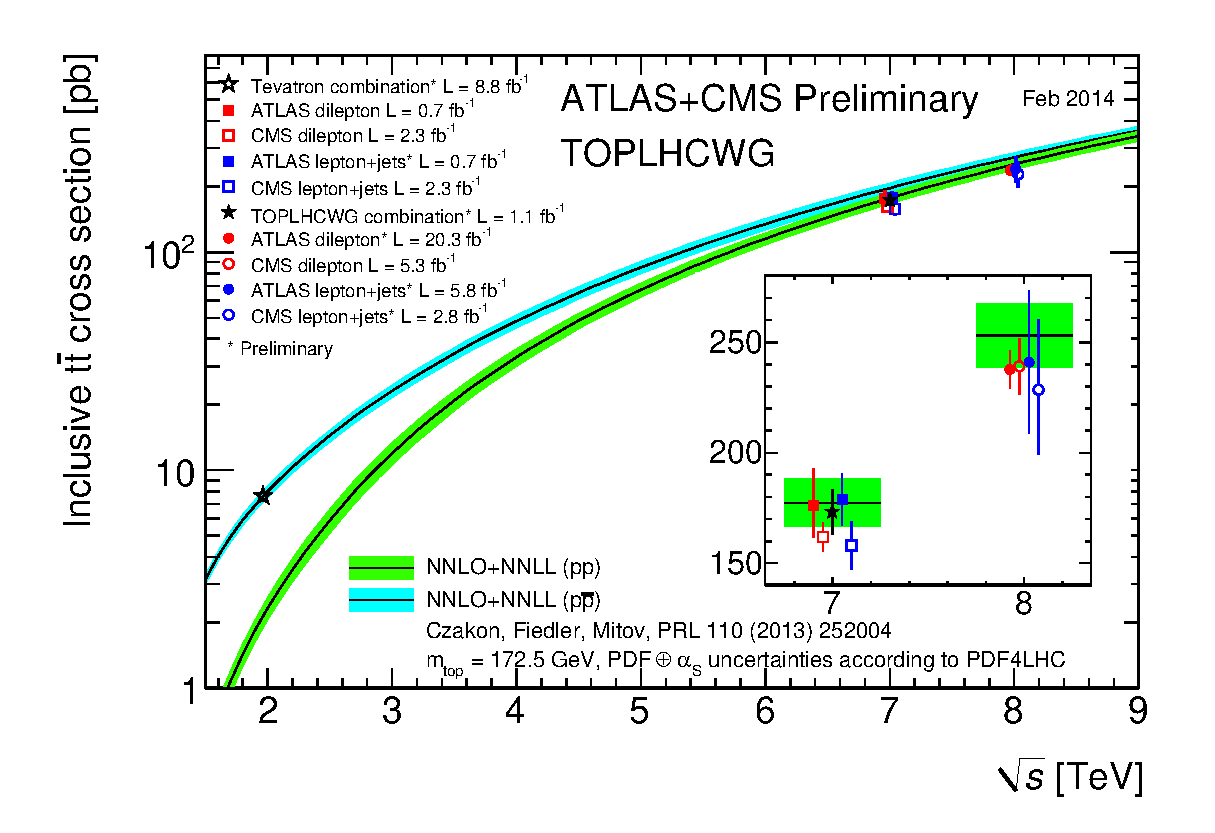
\includegraphics[width=0.75\textwidth]{PartTopQuark/Plots/tt_xsec_vsroots.eps}
  \caption[A summary of the most precise \ttbar\ production cross section measurements performed at the LHC at $\sqrt{s}=$ 7 and 8 TeV and the Tevatron at $\sqrt{s}=\SI{1.96}{\TeV}$ compared to the theoretical prediction.]{A summary of the most precise \ttbar\ production cross section measurements performed at the LHC at $\sqrt{s}=$ 7 and 8 TeV and the Tevatron at $\sqrt{s}=\SI{1.96}{\TeV}$ compared to the theoretical prediction~\cite{TopQuark:SummaryPlots}. The Tevatron results should be compared against the prediction for $p\bar{p}$ collisions while the LHC against the $pp$ collision predictions.}\label{fig:TopQuarkPairProductionComparison}
\end{figure}

\subsubsection{Top mass measurement}

The mass of the top $m_{t}$ is a fundamental parameter of the SM\@. Measurements of the top mass have been carried out in all \ttbar\ channels at both ATLAS and CMS~\cite{Top:TopMassCombination}. These results are summarized in Figure~\ref{fig:TopQuarkMtopSummaryATLAS}, which includes the combined LHC measurement:
%
\begin{equation*}
  m_{t}=173.29\pm0.23\stat\pm0.92\syst\si{\GeV}
\end{equation*}

\begin{figure}[htbp]
  \centering
  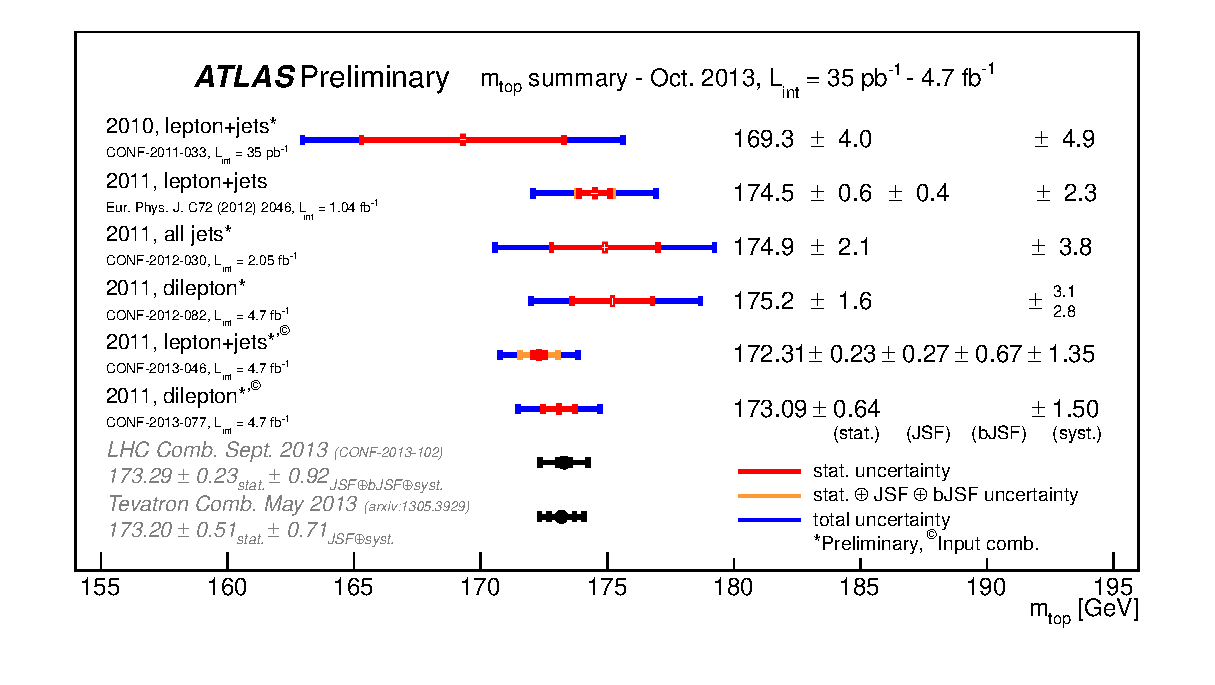
\includegraphics[width=0.75\textwidth]{PartTopQuark/Plots/mtopHistory_ATLASAll.eps}
  \caption[Summary of all $m_{t}$ measurement results per analysis at ATLAS.]{Summary of all $m_{t}$ measurement results per analysis at ATLAS~\cite{TopQuark:SummaryPlots}. The statistical combination of these results are compared to the combination from Tevatron.}\label{fig:TopQuarkMtopSummaryATLAS}
\end{figure}

\subsubsection{Boosted top resonance searches}

Some BSM theories predict the existence of additional particles with large masses that can decay into a pair of top quarks with very large transverse momenta. The decay products of these highly boosted tops emerge in a collimated cone. Boosted top searches have been carried out at ATLAS~\cite{Boosted:ATLASExclusion7TeV}, looking for the decay products of a heavy boson known as the $Z'$~\cite{TopQuark:TC2,TopQuark:TC22,TopQuark:ZPrimeCross} and Kaluza-Klein gluons~\cite{TopQuark:KKGluonTwo,TopQuark:KKGluonOne,TopQuark:KKGluonThree,TopQuark:KKGluonFour,TopQuark:KKGluonFive}. A narrow leptophobic $Z'$ with a mass of less than \SI{1.74}{\TeV} is excluded and a Kaluza-Klein gluon is excluded for masses below \SI{2.07}{\TeV} as shown in Figure~\ref{fig:BoostedLimits}.

\begin{figure}[htbp]
  \centering
  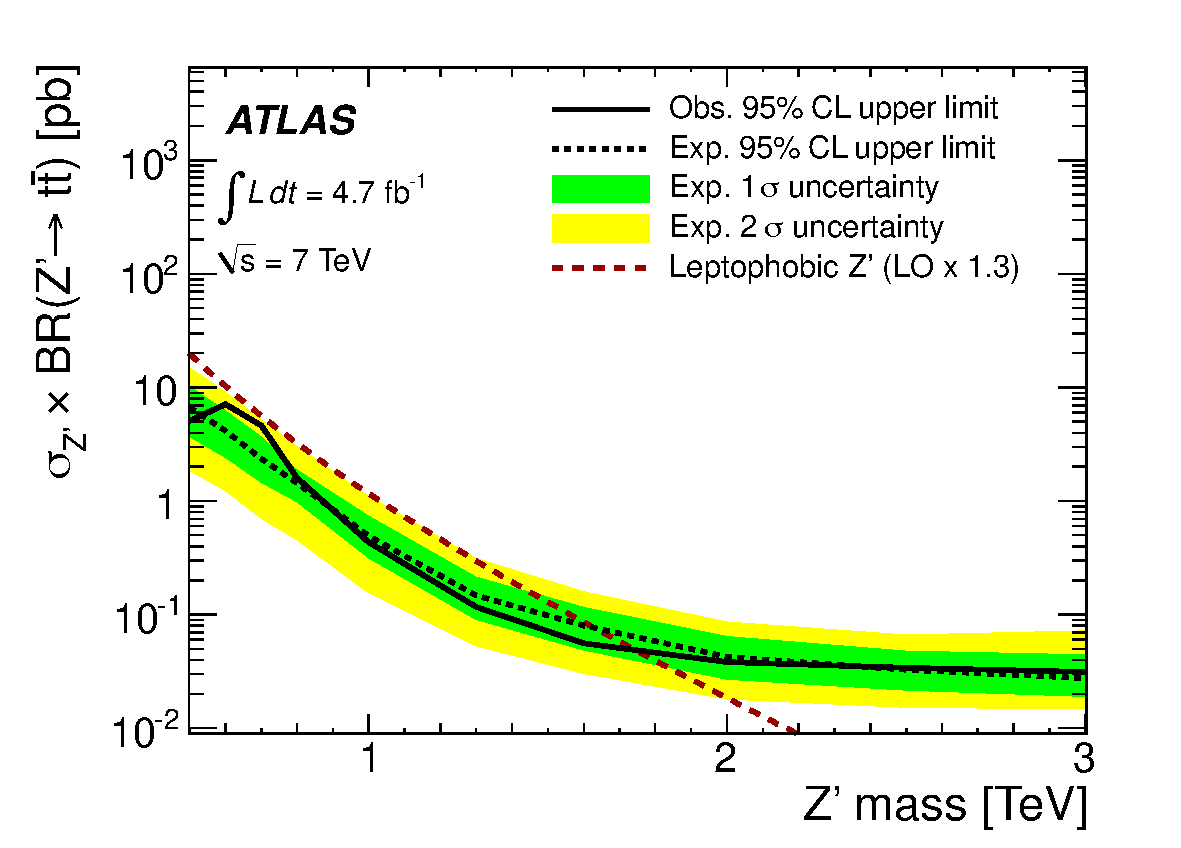
\includegraphics[width=0.75\textwidth]{PartTopQuark/Plots/fig_11a.pdf}

  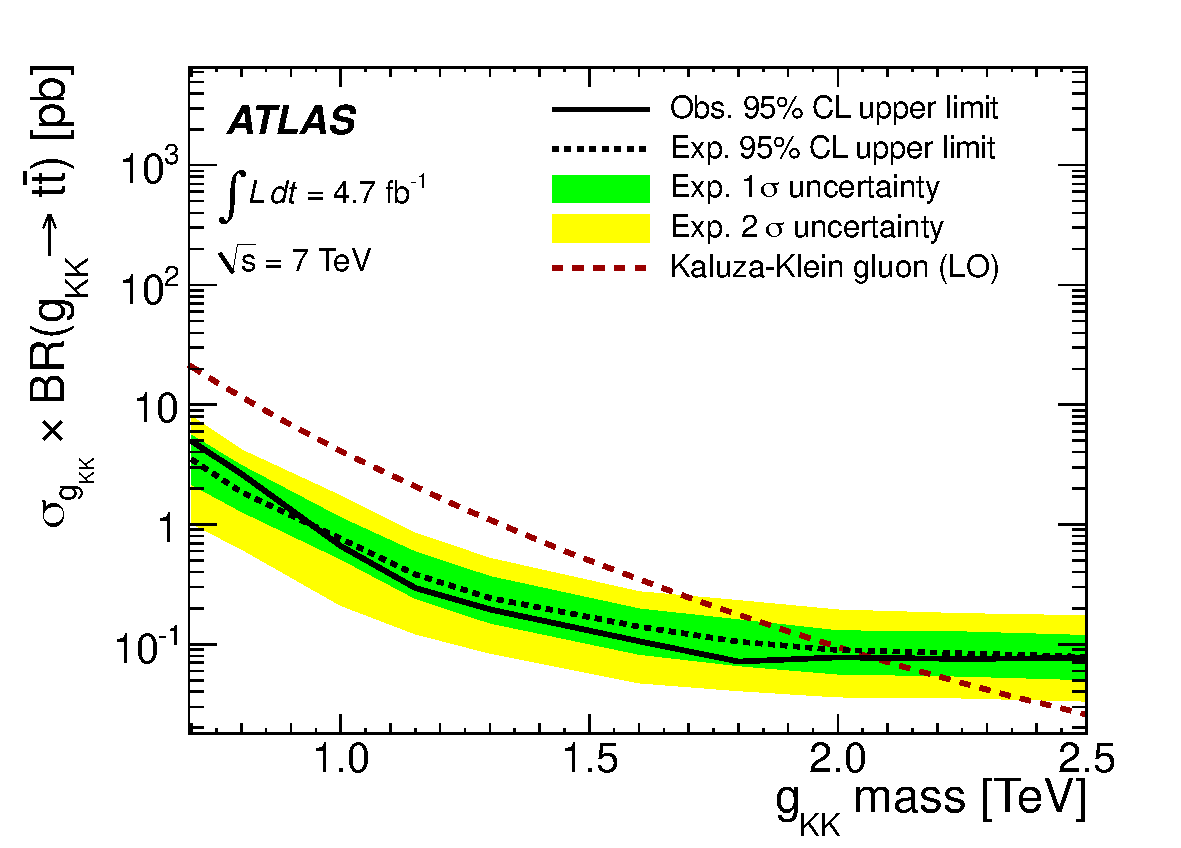
\includegraphics[width=0.75\textwidth]{PartTopQuark/Plots/fig_11b.pdf}
  \caption[Expected (dashed line) and observed (solid line) upper limits on the cross section times the \ttbar\ branching ratio of \Zprime\ (left) and Kaluza-Klein gluons (right) using the combined resolved and boosted selections.]{Expected (dashed line) and observed (solid line) upper limits on the cross section times the \ttbar\ branching ratio of \Zprime\ (left) and Kaluza-Klein gluons (right) using the combined resolved and boosted selections. The dark (green) and light (yellow) bands show the range in which the limit is expected to lie in \SI{68}{\percent} and \SI{95}{\percent} of pseudo-experiments, respectively, and the smooth solid (red) lines correspond to the predicted cross section times branching fraction. Both statistic and systematic uncertainties have been included~\cite{Boosted:ATLASExclusion7TeV}.}\label{fig:BoostedLimits}
\end{figure}

